\documentclass[a4paper, 11pt]{report}
\usepackage[T1]{fontenc} % Caractere francais
\usepackage[utf8]{inputenc}
\usepackage[english,french]{babel} 
\usepackage{graphicx} % Pour les images
\def\@captype{figure}
\usepackage{float}
\usepackage{multicol} % Pour faire des multi colonnes
\usepackage[export]{adjustbox} % Pour la clé 'valign'  (aligner verticalement)
\usepackage[colorlinks=true,linkcolor=black]{hyperref} % Pour qu'il y est des liens sur la table des matières
\usepackage{caption} % Utiliser plus de fonction sur caption (caption* pour ne pas afficher FIGURE-1)
\usepackage{lipsum} % Pour générer du texte pour voir comment ca rend
\usepackage{ragged2e} % Pour justifier le texte
\usepackage{ulem}
\usepackage[margin=3.2cm]{geometry}
\usepackage{forest}
\usepackage{listings}
\usepackage{xcolor}
\usepackage[section]{placeins}
\usepackage{amsmath}
\usepackage{amssymb}
\usepackage{fancybox}
\usepackage{fancyhdr}
\usepackage{url}
\usepackage{appendix}
\usepackage{texnames}



% Définir une couleur pour les citations
\definecolor{citationcolor}{rgb}{0.0, 0.5, 1.0}  % Couleur bleue par exemple

% Modifier la couleur des citations
\hypersetup{
    citecolor=citationcolor  % Applique la couleur aux citations
}

% Configuration de fancyhdr
\pagestyle{fancy}
\fancyhf{} % Efface tous les en-têtes et pieds de page précédents
\fancyhead[C]{Rapport de projet} % Texte centré en haut de la page
\fancyfoot[L]{2024-2025} % Texte en bas à gauche du pied de page
\fancyfoot[C]{Samia BENALI \& Elouan BOITEUX} % Texte au centre du pied de page
\fancyfoot[R]{\thepage} % Numéro de page en bas à droite du pied de page

\renewcommand{\headrulewidth}{0.4pt} % Épaisseur de la ligne de séparation de l'en-tête
\renewcommand{\footrulewidth}{0.4pt} % Épaisseur de la ligne de séparation du pied depage
\setlength{\headheight}{13.59999pt}
% Appliquer le style d'en-tête fancy aux pages de début de chapitre

\fancypagestyle{plain}{
  \fancyhf{} % Effacer tous
  \fancyhead[C]{Rapport de Stage} % Texte centré en haut de la page
  \fancyfoot[L]{L2 CMI Informatique} % Texte en bas à gauche du pied de page
  \fancyfoot[C]{Samia BENALI \& Elouan BOITEUX} % Texte au centre du pied de page
  \fancyfoot[R]{\thepage} % Numéro de page en bas à droite du pied de page
  \renewcommand{\headrulewidth}{0.4pt} % Épaisseur de la ligne de séparation de l'en-tête
  \renewcommand{\footrulewidth}{0.4pt} % Épaisseur de la ligne de séparation du pied de page
}


\newcommand{\annotation}[1]{\colorbox{yellow}{#1}}

\newcommand{\var}[1]{\texttt{\textbf{#1}}}
\newcommand{\langage}[1]{\texttt{#1}}


\usepackage{tocloft}
\setlength{\cftbeforetoctitleskip}{1.5cm}  % Ajuste l'espace avant le titre de la table des matières


\begin{document}


% Première page
\begin{titlepage}
	\centering
	% \vspace*{2cm}
	{\Huge \textbf{Université de Franche-Comté} \par}
	\vspace{1cm}
	{\huge \texttt{}{Projet d'Initiation à la recherche\\ } \LARGE{\textbf{L2 - CMI}} \par}
	\vspace{1cm}
	{\huge \textbf{Complétion (semi-)automatique} \par}
	\vspace{1cm}
	{\Large BOITEUX Elouan\\BENALI Samia\par}
	\vspace{0.5cm}
	\begin{center}
		{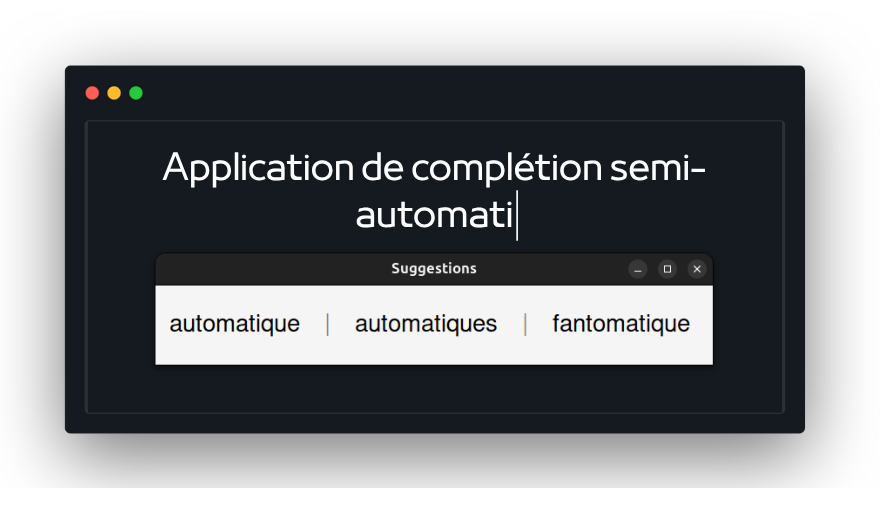
\includegraphics[height=0.55\textwidth]{images/illustration.png}}
	\end{center}

	\begin{minipage}[c]{0.40\textwidth}
		\centering
		\raisebox{-0.5\height}{
\includegraphics[width=\textwidth]{images/logo_univ.png}}
	\end{minipage}
	\hfill
	\begin{minipage}[c]{0.5\textwidth}
		\centering
		\raisebox{-0.5\height}{
\includegraphics[width=\textwidth]{images/logo_CMI.png}}
	\end{minipage}
	\vfill
	{2024/2025}
\end{titlepage}

\chapter*{Remerciements}
\addcontentsline{toc}{chapter}{Remerciements}

Nous souhaiterions remercier dans un premier temps Pierre-Cyril HEAM de nous avoir permis d'effectuer un projet semestriel sur la complétion semi-automatique et de nous avoir encadré tout au long du semestre. \\

Nous souhaiterions également remercier chaleureusement Jean-Michel HUFFLEN de nous avoir appris le langage \LaTeX{} pour la rédaction de nos rapports ainsi que tous les professeurs que nous avons rencontrés et qui nous ont permis d'acquérir nos connaissances actuelles sur les langages utilisés.\\

Nos remerciements vont également à toutes les personnes avec lesquelles nous avons pu discuter et partager autour des projets de recherches et tout spécialement les étudiants du CMI Informatique pour leur gentillesse et leur aide précieuse. \\



\newpage
\tableofcontents



\chapter*{Introduction} % * pour ne pas avoir de numéro de chapitre
\addcontentsline{toc}{chapter}{Introduction}

Dans le cadre de notre projet de recherche du CMI informatique de l’Université de Marie \& Louis Pasteur de Besançon, encadré par Monsieur Héam, nous avons travaillé sur la complétion (semi-)automatique.\par \vspace{\baselineskip} % pour une ligne vide


Ce projet nous a permis de découvrir ce qu'était la complétion automatique et la complétion semi-automatique et de comprendre sur quoi ce repose ces deux notions. La complétion automatique est un processus par lequel un système va prédire et compléter une entrée en fonction de certaines données et contextes. Cependant, la complétion semi-automatique, est une assistance permettant au système de proposer des options tout en laissant à l'utilisateur la décision finale. La complétion (semi-)automatique peut être utilisée dans de nombreuses applications : une saisie sur clavier, une complétion de code, une recherche sur un moteur de recherche, une assistance virtuelle etc\dots\par \vspace{\baselineskip} % pour une ligne vide


Ce rapport va nous permettre, dans un premier temps, d’étudier les différentes approches qui existent ainsi que  les différents algorithmes de distance. Ensuite, nous parlerons  des chaînes de Markov pour la gestion d'historique et enfin vous retrouverez l'application que nous avons créer permettant une complétion semi-automatique.\par
\vfill

\chapter{Les différentes approches utilisées}

\section{Modèles s'appuyant sur des règles}
Pour proposer des suggestions, ce modèle utilisent des algorithmes simples qui s'appuient sur des règles préprogrammées telles que la correspondance de préfixes ou une séquence donnée en amont. Ces algorithmes vont être gérer principalement grâce à des dictionnaires statiques ou des listes.  Cette implémentation est plutôt rapide et simple à mettre en place, elle est cependant très peu flexible et empêche donc une utilisation complexe\dots

\section{Modèles s'appuyant sur des statistiques}
Pour proposer des suggestions, ce modèle utilisent des statistiques fournies grâce aux données d'un historique. Cela permettra de prédire des séquences comme avec le modèle de Markov (expliqué dans le chapitre \ref{Markov}) ou la méthode TF-IDF \textit{(term frequency-inverse document frequency)}
Cette implémentation permet d'obtenir des résultats rapidement. On a cependant aucune compréhension sémantique donc les suggestions ne conviendront que rarement au contexte\dots

\section{Modèles s'appuyant sur l'intelligence artificielle}
Pour proposer des suggestions, ce modèle utilisent des algorithmes qui s'appuient sur l'intelligence artificielle et les réseaux neuronaux.
Avec l’apprentissage supervisé et non supervisé, ces modèles apprennent des motifs complexes à partir des données. Ils peuvent inclure des algorithmes comme les forêts aléatoires ou les régressions pour fournir des prédictions plus contextuelles.
Cette implémentation permet d'être efficace face à des problèmes très complexes et de répondre à des demandes rares. Cependant, ce genre d'implémentation nécéssite énormément de temps de calculs et de ressources\dots
\newpage

\section{Modèles s'appuyant sur le deep learning}
Pour proposer des suggestions, ce modèle utilise des algorithmes qui s'appuient sur l'amélioration en temps réel. C'est à l'utilisateur de faire des choix et ces mêmes choix sont mémorisés pour une utilisation personnalisée et plus précise. Cette implémentation est donc très adapatable et permet des réponses précises avec un sens sémentique. Cependant, cette implémentation est complexe et très longue à mettre en place puisque les choix de l'utilisateur sont nécessaires et les réponses dépendront en grande partie des données collectées\dots



\chapter{Les algorithmes de calcul de distance}

\section{Introduction}

Un algorithme de calcul de distance permet de mesurer la similarité et/ou la différence entre deux objets tels que du textes, des vecteurs, des chaînes de caractères. On utilise ces algorithmes de calcul principalement pour la correction d'orthographe, le traitement de texte, les alignements de séquences ADN ou encore pour la recherche d'informations.

\section{Distance d'édition ou de Levenshtein}

L'algorithme de calcul de distance d'édition permet de rechercher le nombre minimal d'opérations élémentaires, tels que les insertions, les suppressions et les substitutions, qui seront nécessaires à la transformation d'une chaîne de caractères en une autre. L'insertion permet d'ajouter un caractère, la suppression d'en enlever, et la subtitution d'en replacer un caractère par un autre. La figure~\ref{fig:levenshtein} montre un exemple d'illustration de ces opérations. \par \vspace{\baselineskip}

La compexité de l'algorithme est en $\mathcal{O}(n \times m)$  où n est la longueur de la première chaîne et m la longueur de la seconde. Sa complexité dans l'espace est équivalente. Dans certaines implémentations avancées, la complexité dans l'espace peut être réduite à $\mathcal{O}(\min(n,m))$. \par \vspace{\baselineskip}

Il s'agit d'une implémentation simple et intuitive qu'il est facile de mettre en place. Cependant, elle ne prend pas en compte les permutations et ne peut pas résoudre des erreurs plus complexes que l'insertion, la suppression et la subtitution.


\begin{figure}[H]
	\begin{center}
		{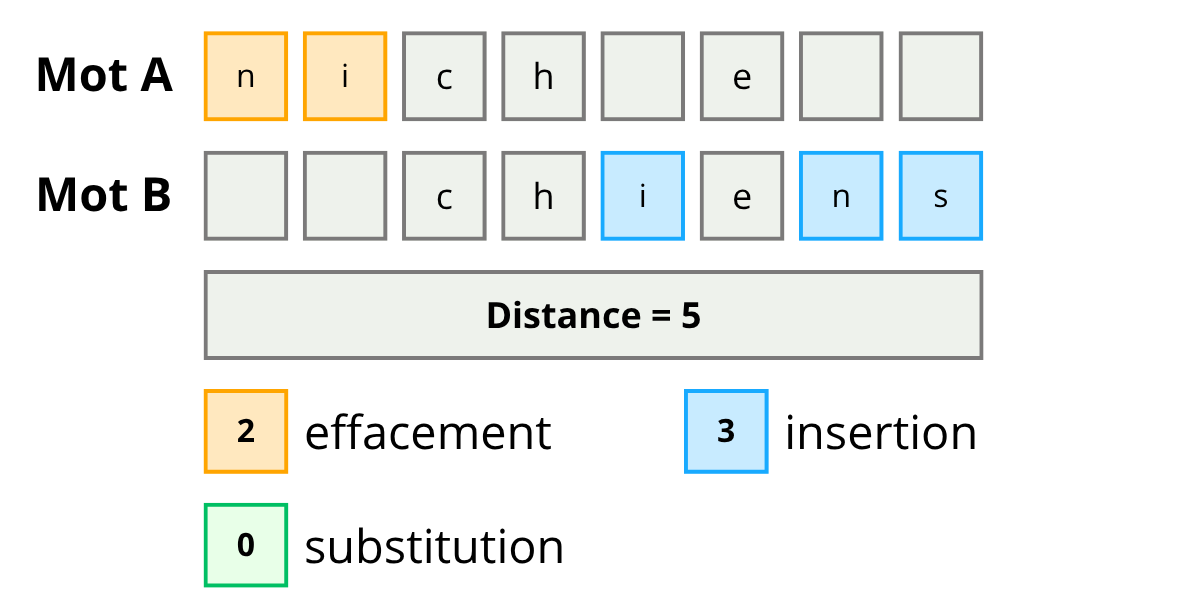
\includegraphics[height=0.45\textwidth]{images/levenshtein.png}}
	\end{center}
	\caption{Exemple distance de Levenshtein}
	\label{fig:levenshtein}
\end{figure}

\noindent{}La formule du calcul de la distance de Levenshtein est la suivant :

\[
	\text{lev}(a, b) =
	\begin{cases}
		\max(|a|, |b|)           & \text{si } \min(|a|, |b|) = 0, \\
		\text{lev}(a - 1, b - 1) & \text{si } a[0] = b[0],        \\
		1 + \min \begin{cases}
			         \text{lev}(a - 1, b) \\
			         \text{lev}(a, b - 1) \\
			         \text{lev}(a - 1, b - 1)
		         \end{cases} & \text{sinon}.
	\end{cases}
\]

\vspace{\baselineskip}
\noindent{}On cherche le nombre minimal d'opérations pour transformer la chaîne \var{a} en chaine \var{b}.

\section{Distance de Damerau-Levenshtein}

L'algorithme de calcul de distance de Damerau-Levenshtein permet de faire la même chose que l'algorithme de calcul de distance de Levenshtein en y ajoutant l'opération de transposition de deux caractères adjacents.  \\

Les complexités en temps et dans l'espace de l'algorithme restent les mêmes que la distance de Levenshtein. Cependant, même dans les implémentations avancées, la complexité dans l'espace ne peut pas être réduite. \\

Il s'agit d'une implémentation qui reste simple et intuitive et qui, de plus, a une meilleure gestion des erreurs de type (\og{}ab\fg{} et \og{}ba\fg{}). Elle est toute fois plus coûteuse que Levenshtein.

\begin{figure}[H]
	\begin{center}
		{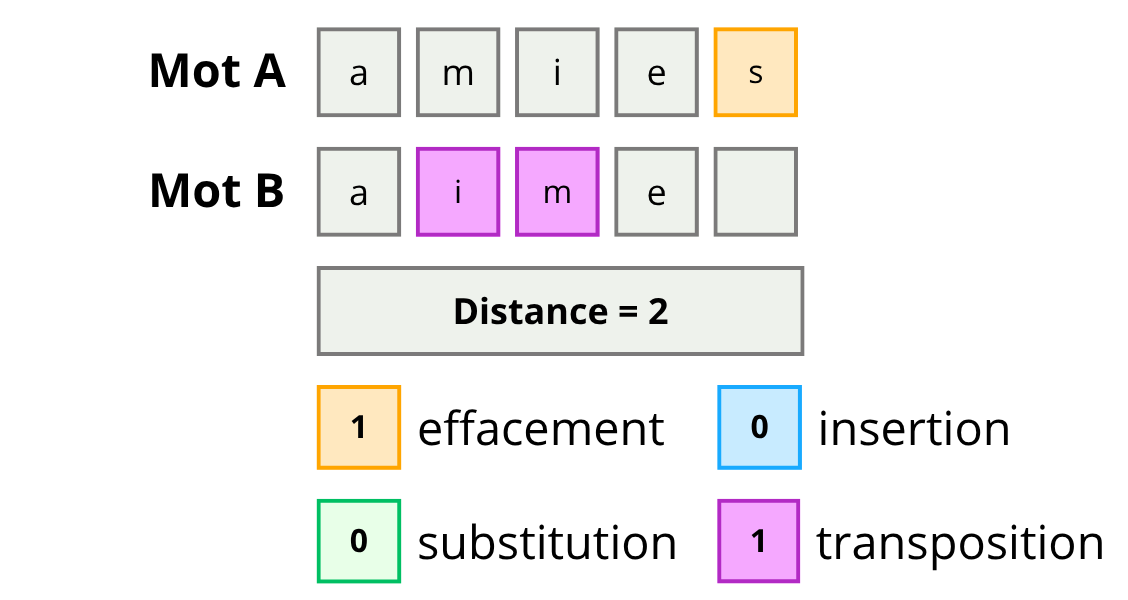
\includegraphics[height=0.45\textwidth]{images/damerau-levenshtein.png}}
	\end{center}
	\caption{Exemple distance de Damerau-Levenshtein}
	\label{fig:damerau}
\end{figure}
\section{Distance de Hamming}

L'algorithme de calcul de distance de Hamming va rechercher, dans deux chaînes de même longueur, le nombre de positions qui vont différer. La figure~\ref{fig:hamming} montre un exemple de ce calcul de distance.\\

Les complexités en temps et dans l'espace de l'algorithme sont en $\mathcal{O}(n)$ où n est la longueur des deux chaînes. \\

C'est un algorithme facile à implémenter et très rapide. Cependant, il ne fonctionne que sur des chaînes de même longueur ce qui peut vite s'avérer restrictif.\\

\begin{figure}[H]
	\begin{center}
		{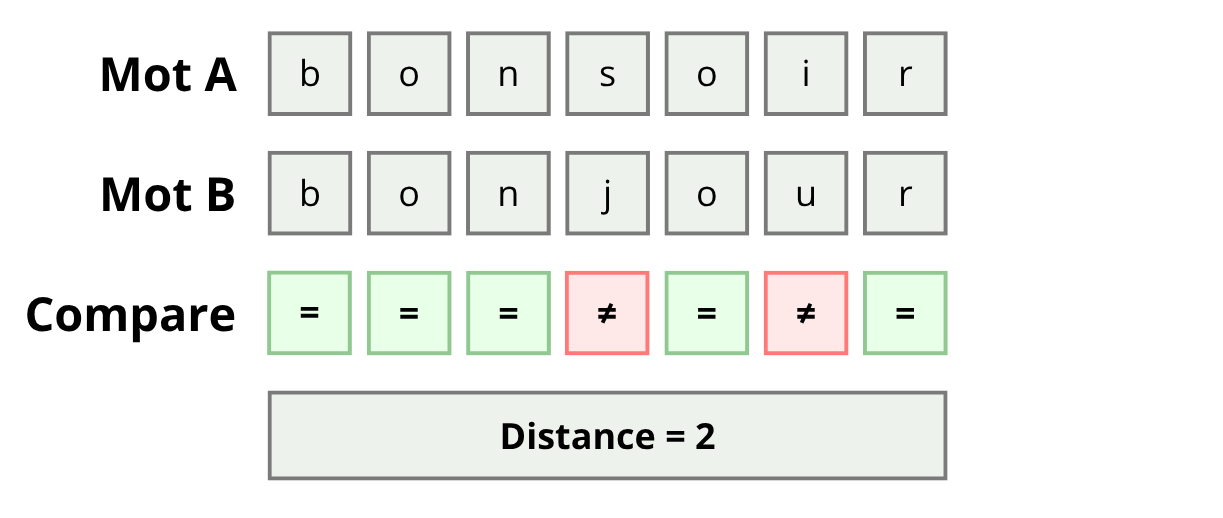
\includegraphics[height=0.4\textwidth]{images/hamming.png}}
	\end{center}
	\caption{Exemple distance de Hamming}
	\label{fig:hamming}
\end{figure}


\chapter{Chaine de Markov}
\label{Markov}
\section{Définition}

Une chaîne de Markov est un modèle mathématique qui représente un sytème où la probabilité de passer d'un état à un autre dépend uniquement de l'état actuel. Les états sont les différents éléments du système. Les transitions sont les différentes probabilités de passer d'un état à un autre. \par
Une matrice de transition est une table qui permet de regrouper les probabilités de transition entre tous les états.

\section{Application}
On utilise les chaînes de Markov pour modéliser des processus aléatoires, pour analyser des séquences données, des prédictions ou encore des historiques de navigation. Nous allons nous concentrer sur les historiques de navigation sur le web ainsi que l'historique des actions de l'utilisateur. \\

Imaginons qu'un utilisateur navigue entre trois pages web A, B et C. \\
Alors une chaîne de Markov pourrait ressembler à :


\begin{table}[h!]
	\centering
	\begin{tabular}{|c|c|c|}
		\hline
		\textbf{Depuis} & \textbf{Vers} & \textbf{Probabilité} \\
		\hline
		A               & B             & 0.6                  \\
		A               & C             & 0.4                  \\
		B               & A             & 0.3                  \\
		B               & C             & 0.7                  \\
		C               & A             & 0.5                  \\
		C               & B             & 0.5                  \\
		\hline
	\end{tabular}
	\caption{Probabilités de transition entre les états}
\end{table}


\newpage
La matrice de transition serait donc :

\[
	M =
	\begin{bmatrix}
		0   & 0.6 & 0.4 \\
		0.3 & 0   & 0.7 \\
		0.5 & 0.5 & 0
	\end{bmatrix}
\]


L'objectif serait d'utiliser l'historique de navigation ou l'historique des actions de l'utilisateur pour modéliser les transitions probables entre les différentes étapes. \\
Pour cela, on doit premièrement collecter les données des historiques. Ensuite, on compte les transitions observées entre les états pour calculer les probabilités de transition. Enfin, on construit la matrice de transition.

\section{Exemple}

\noindent{}Prenons l'exemple de l'historique suivant :
\[
	A \Longrightarrow C \Longrightarrow B \Longrightarrow A \Longrightarrow B \Longrightarrow C
\]

\noindent{}La première chose a faire est d'observer le nombre de transitions :
\begin{table}[h!]
	\centering
	\begin{tabular}{|c|c|c|}
		\hline
		\textbf{Depuis} & \textbf{Vers} & \textbf{Nombre d'observations} \\
		\hline
		A               & C             & 1                              \\
		C               & B             & 1                              \\
		B               & A             & 1                              \\
		A               & B             & 1                              \\
		B               & C             & 1                              \\
		\hline
	\end{tabular}
	\caption{Transitions observées et leur fréquence}
\end{table}

Ensuite, il faut calculer les probabilités de transition. \\
Pour ce faire, on considère la probabilité de transition entre deux états \(X\) et \(Y\). Il s'agit de compter le nombre de fois où la transition de \(X\) vers \(Y\) a été observée, puis de diviser ce nombre par le total des transitions partant de l'état \(X\).

\subsection*{Transitions depuis A}
\begin{itemize}
	\item Transitions observées : \( A \rightarrow C \), \( A \rightarrow B \)
	\item Nombre total de transitions depuis A : \(2\)
	\item Probabilités :
	      \begin{itemize}
		      \item \( P(A \rightarrow C)  = 0.5 \)
		      \item \( P(A \rightarrow B)  = 0.5 \)
	      \end{itemize}
\end{itemize}o

\subsection*{Transitions depuis B}
\begin{itemize}
	\item Transitions observées : \( B \rightarrow A \), \( B \rightarrow C \)
	\item Nombre total de transitions depuis B : \(2\)
	\item Probabilités :
	      \begin{itemize}
		      \item \( P(B \rightarrow A) = 0.5 \)
		      \item \( P(B \rightarrow C) = 0.5 \)
	      \end{itemize}
\end{itemize}

\subsection*{Transitions depuis C}
\begin{itemize}
	\item Transition observée : \( C \rightarrow B \)
	\item Nombre total de transitions depuis C : \(1\)
	\item Probabilité :
	      \begin{itemize}
		      \item \( P(C \rightarrow B) = 1 \)
	      \end{itemize}
\end{itemize}

\subsection*{Matrice de transition}
On obtient donc une matrice de transition.

\[
	M =
	\begin{bmatrix}
		0   & 0.5 & 0.5 \\
		0.5 & 0   & 0.5 \\
		0   & 1   & 0
	\end{bmatrix}
\]



\section{Conclusion}
Les chaînes de Markov permettent de prédire l'étape suivante en se basant sur les actions précédentes. Cela va permettre, par la suite, de personnaliser les suggestions pour chaque utilisateur. \par
De plus, ce système est facile à mettre en place et à implémenter. Cependant, une chaîne de Markov ne prend pas en compte l'historique complet ce qui mène à un problème de mémoire. Il faut, de plus, un très grand nombre de données et un historique plus grand pour avoir des données fiables .
\chapter{Notre outil de complétion (semi-)automatique}

\section{Choix pour l'implémentation}

Tout d'abord, nous avons dû choisir un langage de programmation pour implémenter ce projet semestriel. Il nous fallait un langage permettant de minimiser le temps de calculs de la distance, entre les mots avec lesquels nous travaillons. De plus, nous souhaitions utiliser cette occasion pour découvrir un nouveau langage.~{\langage{Rust} s’est donc révélé plus adapté que les autres langages, puisqu’il offre une excellente vitesse de calcul et limite donc considérablement la latence.\\

Nous devions ensuite mettre en place le projet. Nous avons décider d'à la fois recréer une interface de suggestions de mots comme sur les téléphones portables mais sur ordinateur, et que l'application soit utilisable sur \langage{Ubuntu} et depuis n'importe quelles applications. En effet, créer une application qui suggère des mots mais qui n'est pas utilisable dans d'autres applications n'est pas d'un grand interêt.

\section{Les étapes de la réalisation}

\subsection{Keylogger \& mouselogger}
Dans un premier temps, nous voulions pouvoir récupérer tous les évènements clavier de l'utilisateur quelque soit l'application sur laquelle il se trouve. La solution retenue pour ce projet a été de développer un keylogger. Un keylogger (ou enregistreur de frappe) est un programme qui s’exécute en arrière-plan de l'ordinateur et récupère les frappes de l’utilisateur sur son clavier. Après la détection de chaque touche pressée, notre keylogger traduit l'identifiant reçu en caractère grâce au fichier \textbf{/usr/include/linux/input-event-codes.h} que l'on retrouve dans les fichiers de l'\langage{OS}. Ce fichier associe une touche (lettre I par exemple) en un identifiant (23 pour I). La figure~\ref{fig:lecture_touche} montre un extrait de ce fichier. On utilise donc l'identifiant, que l'on traduit à nouveau, et cela permet ainsi de construire le mot au fur et à mesure. \\

\begin{figure}[H]
	\begin{center}
		{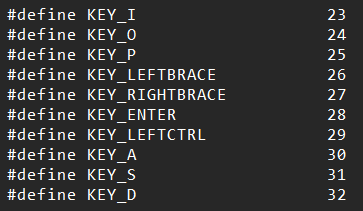
\includegraphics[width=0.6\textwidth]{images/fichier_touche.png}}
	\end{center}
	\caption{Extrait du fichier input-event-codes.h}
	\label{fig:lecture_touche}
\end{figure}

En plus des touches alphanumériques, notre programme gère également certaines touches spéciales comme les flèches directionnelles. Lorsqu’une flèche gauche ou droite est détectée, le keylogger met à jour la position du curseur dans le mot en cours de construction. Ainsi, lorsqu’une nouvelle lettre est tapée après un déplacement avec les flèches, elle est insérée à la bonne position dans la chaîne, et non simplement ajoutée à la fin. Cela permet de refléter fidèlement l’intention de l’utilisateur, même s’il modifie le mot partiellement avant de le terminer. Ce comportement permet à notre programme de reconstituer précisément les mots saisis, y compris avec des corrections ou insertions en milieu de mot.



Une fois ajouté à notre programme principal, nous pouvons désormais récupérer les frappes de l'utilisateur. Grâce à cela, nous pouvons désormais concaténer les lettres et afficher dans un terminal le mot en cours de saisie. Pour une utilisation plus fluide, nous avons ajouté quelques fonctionnalités supplémentaires. Notre programme gère également certaines touches spéciales comme les flèches directionnelles. Lorsque la flèche gauche ou droite est détectée, le keylogger met à jour la position du curseur dans le mot en cours de construction. Ainsi, lorsqu’une nouvelle lettre est tapée après un déplacement avec les flèches, elle est insérée à la bonne position dans la chaîne, et non simplement ajoutée à la fin. Cela permet de refléter fidèlement l’intention de l’utilisateur, même s’il modifie le mot partiellement avant de le terminer. Ce comportement permet à notre programme de reconstituer précisément les mots saisis, y compris avec des corrections ou insertions en milieu de mot. De plus, s'il clique sur la touche retour arrière, il peut supprimer la lettre à gauche du curseur sans que notre programme perde l'information du mot en cours de saisie. Enfin si l'utilisateur clique sur n'importe quelle autre touche qu'une lettre (accentuée ou non), le retour arrière ou les flèches de navigation alors, on annule les suggestions de mots. \\

Nous avons décider d'ajouter une détection de clics de souris afin d'annuler la proposition de suggestions lorsque l'utilisateur n'a plus le curseur de texte sur le mot qu'il est en train d'écrire. Cette implémentation a été simple et rapide puisque nous reprenons le même principe que le keylogger. \\

Une fois cette première partie terminée, nous avons constater que notre programme détectait qu'un seul clavier et qu'une seule souris. Or, si un utilisateur utilise un ordinateur portable et y branche un clavier externe, notre détection de saisie de fonctionne plus. \\

La principale difficulté a été de détecter tous les claviers et souris puis de les faire fonctionner en même temps. On a décidé d'utiliser des threads pour lire les fichiers des claviers et des souris en concurrence. Un thread est une séquence d'instructions qui pourra être exécutée indépendamment au sein d'un programme. Les threads permettent une exécution simultanée et un fonctionnement multitâche au sein d'une même application. La figure~\ref{fig:lecture_fichier} montre un schéma de la lecture des fichiers en concurrence grâce aux threads.

\begin{figure}[H]
	\begin{center}
		{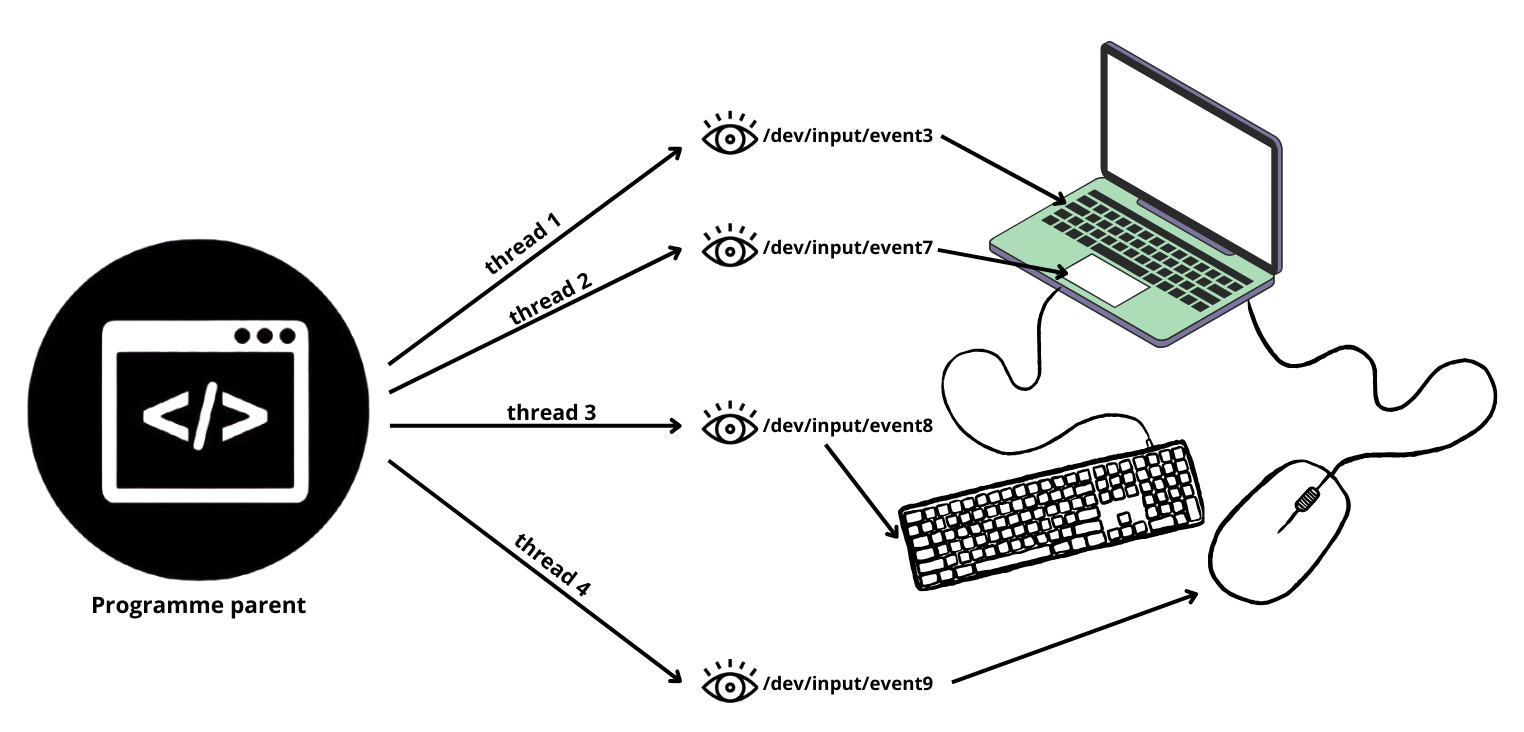
\includegraphics[width=\textwidth]{images/lecture-fichier.png}}
	\end{center}
	\caption{Schéma descriptif des lectures fichiers}
	\label{fig:lecture_fichier}
\end{figure}

Cependant, il restait un problème : arrêter proprement notre programme. En effet, lorsque l'on ferme l'interface graphique, les threads sont encore en train de lire les fichiers des claviers et des souris et ils ne se ferment donc pas. Pour pallier ce problème, nous avons fait en sorte qu'un signal soit envoyé à notre code \langage{Rust} lorsque l'interface graphique \langage{Python} est fermée. Lorsque le signal est reçu, ce dernier l'envoie aux threads qui sont gérés de façon asynchrones et qui ferment ainsi la lecture du fichier. Pour que les signaux permettent d'arrêter la lecture des fichiers de périphériques, nous avons dû modifier la structure de notre code. On obtient ainsi une façon plus propre de fermer le programme.

\subsection{Ecrire et remplacer un mot}

Pour cette deuxième étape, nous devions faire en sorte de pouvoir écrire un mot dans n'importe quelle application, et cela de façon automatique via notre code. Pour ce faire,  noux avons mit en place un clavier virtuel pour simuler les frappes de l'utilisateur et ainsi écrire le mot demandé. Notre code fonctionne ainsi : On crée une fonction permettant de traduire un caractère en l'évènement clavier correspondant. Ensuite, on crée une fonction permettant de cliquer sur un de ces caractères sur le clavier virtuel. Enfin, on répète cette opération avec chaque lettre du mot pour l'écrire en entier.\\

Lorsque cela a été mis en place, on s'est rendu compte que les lettres précédemment écrites par l'utilisateur n'étaient pas effacées. Pour cela, nous avons simplement utilisé la fonction permettant de cliquer sur une touche du clavier virtuel que l'on a lance \textbf{n} fois sur la touche retour arrière (où \textbf{n} est la longueur du mot écrit par l'utilisateur). Comme tout est automatique, le remplacement du mot est instantané, non visible par l'utilisateur et la réécriture reste fluide et naturelle.

\subsection{Algorithme de suggestions}

Maintenant que nous pouvons détecter les frappes de l'utilisateur ainsi qu'écrire et/ou remplacer un mot, nous devons écrire l'algorithme qui nous permettra de faire 3 suggestions à l'utilisateur.\par \vspace{\baselineskip}

Nous avons décidé de nous baser sur un dictionnaire de plus de 140~000 mots trouvé dans \cite{new2019lexique}. Ce dernier est associé à des fréquences d'utilisation que nous utiliserons pour améliorer nos suggestions. Dans un premier temps, nous avons choisi de développer l'algorithme de distance de Levenshtein car il n'a besoin ni d'entraînement ni d'historique pour fonctionner. C'est également le plus simple à mettre en place. Nous avons essayé d'optimisé l'algorithme afin d'avoir le moins d'attente possible entre le moment où l'utilisateur tape sur une touche du clavier et le moment où les suggestions s'affichent. \\

En testant notre algorithme, nous avons donc pris peur puisque, même après notre optimisation, il prenait trop de temps (environ 1 à 2 secondes). Après quelques recherches, nous avons vu qu'il existait  différents profils de compilation tels que : \og debug \fg{} et \og release\fg{}. Durant le développement, nous avons travaillé sur le profil de \og debug \fg{} qui permet une compilation plus rapide mais qui n'est pas optimisé et donc plus lent que le profil \og release \fg. Avec le profil \og release \fg{} l'algorithme s'est déroulé de façon instantanée et était donc utilisable pour notre application.\\

Pour améliorer les suggestions, nous avons décider d'utiliser une des fréquences présentent dans le dictionnaire. (fréquence d'utilisation dans les livres). Nous avons mis en place un algorithme qui permet
\subsection{Interface graphique}

Maintenant que l'algorithme est fonctionnel, nous devons afficher à l'écran les suggestions proposé grâce à une interface graphique. Nous voulions dans un premier temps faire cet interface en \langage{Rust} avec \langage{GTK}, la boîte à outils de \langage{Rust}  mais nous n'avons malheureusement pas réussi à faire en sorte de garder la fenêtre au premier plan lorsque l'utilisateur est sur une autre application. Cette approche devient donc inutilisable car l'application disparait à chaque fois que l'utilisateur clique sur une fenêtre Il ne peut ainsi pas voir les différentes suggestions.\\

On a donc décidé de faire l'interface en \langage{Python} avec Tkinter car nous l'avions déjà utiliser pour d'autres projets et nous savions comment garder la fenêtre au premier plan. Pour ce faire, notre code \langage{Rust} lance un programme \langage{Python} et lui envoie les 3 mots suggérés via l'entrée strandard du code \langage{Python}. Notre code \langage{Python} les affiche dans l'interface. Si l'utilisateur clique sur l'un des trois mots, \langage{Python} envoie l'information au code \langage{Rust} qui va ensuite l'écrire dans l'application de l'utilisateur grâce à notre clavier virtuel.\\

La plus grosse difficulté de l'interface graphique a été la communication de \langage{Rust} et \langage{Python} mais également de faire en sorte que la page reste au premier plan.\\

La figure~\ref{fig:lecture_fichier} illustre l’interface finale de notre application, développée en \langage{Python} à l’aide de la bibliothèque \langage{Tkinter}.

\begin{figure}[H]
	\begin{center}
		{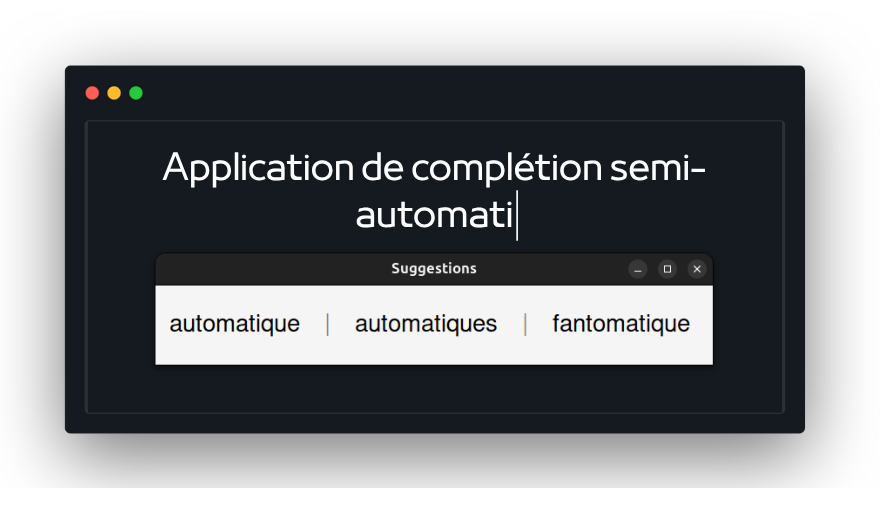
\includegraphics[width=0.7\textwidth]{images/illustration.png}}
	\end{center}
	\caption{Illustration de l'application}
	\label{fig:lecture_fichier}
\end{figure}

\subsection{Installeur de l'application}

Une fois que nous avons tout mis en place et que l'application est fonctionnelle, nous avons décider d'ajouter un installeur d'application qui permet de télécharger toutes les dépendances, d'ajouter l'application dans un dossier contenu dans le \langage{PATH}. Le \langage{PATH} est une variable d'environnement utilisée par le système d'exploitation pour localiser les fichiers exécutables utilisable depuis n'importe quel emplacement dans le systeme.\\

Notre installeur crée aussi un fichier \var{.desktop} pour permettre le lancement l'application depuis le menu d'application d'\langage{Ubuntu} (voir figure~\ref{fig:lanceur}). Il applique également les droits nécessaires aux bons fonctionnements de l'application car certaines commandes nécessitent les droits de l'utilisateur \var{root}, par exemple la lecture des fichiers des périphériques. \\

Nous avons gérer l'installeur grâce à un Makefile, un fichier permettant d'automatiser un ensemble d'actions telles que la génération de fichiers. Nous avons créer une documentation technique pour installer notre application. Vous pouvez la retrouver à l'annexe de la page \underline{\pageref{annexe}}.\\

Grâce à toute cette installation, l'application est plus facile d'accès grâce à une icône dans la barre des taches par exemple.

\begin{figure}[H]
	\begin{center}
		{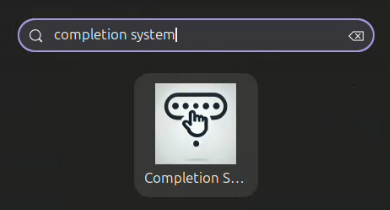
\includegraphics[width=0.5\textwidth]{images/application.png}}
	\end{center}
	\caption{Installeur de l'application}
	\label{fig:lanceur}
\end{figure}

\section{Résultats}
Nous avons donc implémenter une application utilisable sur \langage{Ubuntu} permettant une complétion semi-automatique. Cette application peut se lancer depuis un terminal mais également depuis le gestionnaire d'application d'\langage{Ubuntu}. \par
Une fois l'application lancée, une fenêtre apparait en premier plan et restera toujours en premier plan tant que l'utilisateur ne ferme pas l'application. Si l'utilisateur commence à écrire un mot, trois suggestions seront affichées sur l'interface graphique. Ces suggestions sont calculées grâce à l'algorithme de Levenstein complété avec la gestion des préfixes des mots ainsi que la fréquence d'utilisation des mots proposés. Si l'utilisateur ne veut pas l'un des trois mots proposés, il peut continuer à taper son mot. S'il clique sur l'un des mots, celui-ci sera écrit à la place du mot qu'il était en train d'écrire.


\chapter{Informations complémentaires}

\section{Points à améliorer}

Pour améliorer notre application, nous pourrions faire en sorte qu'elle soit compatible sur d'autres distributions Linux et sur le systeme d'exploitation MacOS. Nous pourrions également changer d'algorithme pour améliorer les suggestions selon l'historique de l'utilisateur par exemple.


\section{Outils utilisés}

Nous avons eu l'occasion d'utiliser de  nombreux outils pour la communication au sein de notre binôme ainsi que pour la réalisation globale du projet semestriel. Nous avons communiquer sur Discord ainsi que sur WhatsApp et partagé l'avancée des projets sur Git. Nous avons également utilisé \langage{Rust}, \langage{Python} et \langage{Tkinter} pour l'implémentation. Enfin le rapport a été rédigé sur \LaTeX{}.

\begin{figure}[H]
	\begin{center}
		{
\includegraphics[width=0.7\textwidth]{images/outils.png}}
	\end{center}
	\caption{Logos des outils utilisés}
	\label{fig:outils}
\end{figure}
\chapter*{Conclusion}
\addcontentsline{toc}{chapter}{Conclusion}
% Page de résumé
\newpage
\begin{center}
	\vspace*{\fill} % Espace vertical
	\section*{Résumé}
	\addcontentsline{toc}{chapter}{Résumé}
	\begin{justify}
		Le resumé


	\end{justify}
\end{center}


\nocite{*}
\bibliographystyle{alpha}
\bibliography{references}

\newpage
\fancypagestyle{annexes}{
	\fancyhf{} % Effacer tous les en-têtes et pieds de page
	\fancyhead[C]{Annexe - Rapport de Stage} % Texte centré en haut de la page
	\fancyfoot[L]{L2 CMI Informatique} % Texte en bas à gauche
	\fancyfoot[C]{Samia BENALI \& Elouan BOITEUX} % Texte au centre
	\fancyfoot[R]{\thepage} % Numéro de page à droite
	\renewcommand{\headrulewidth}{0.4pt} % Ligne de séparation
	\renewcommand{\footrulewidth}{0.4pt} % Ligne de séparation
}

% Appliquer le style "annexes" à partir des annexes
\pagestyle{annexes}  % Appliquer le style "Annexe" à partir de cette page

\addcontentsline{toc}{chapter}{Annexe}
\begin{appendices}  % Démarre la section des annexes
	\begingroup
	\centering
	\section*{Annexe 1 : Documentation technique}
	\label{annexe}
	\endgroup
	\documentclass[11pt,a4paper]{article}
\usepackage[utf8]{inputenc}
\usepackage[T1]{fontenc}
\usepackage[french]{babel}
\usepackage{hyperref}
\usepackage{graphicx}
\usepackage{listings}
\usepackage{xcolor}
\usepackage{geometry}
\geometry{margin=2.5cm}

\title{Documentation technique -- Complétion automatique}
\author{}
\date{}

\begin{document}

\maketitle

\section*{Description générale}

Ce projet implémente un outil de complétion semi-automatique de texte, utilisable dans toutes les applications sur un système Ubuntu.

\section*{Installation}

\subsection*{Prérequis}

\begin{itemize}
	\item Système \textbf{Ubuntu} (testé sur Ubuntu 22.04.2 LTS)
	\item Le raccourci clavier \textbf{Alt + Tab} doit être actif (natif sur Ubuntu) pour changer d'application facilement
\end{itemize}

\subsection*{Étapes d'installation}

\begin{lstlisting}[language=bash]
cd completion-auto/completion-system
make install
\end{lstlisting}

Le \texttt{Makefile} s’occupe de :
\begin{itemize}
	\item Installer les dépendances nécessaires
	\item Copier le binaire compilé dans \texttt{/usr/local/bin/completion-system} (inclus dans le PATH)
	\item Donner les bons droits d’exécution à tous les fichiers nécessaires
\end{itemize}

\section*{Lancement}

Deux méthodes sont possibles :

\begin{itemize}
	\item \textbf{Depuis le terminal} :
	      \begin{lstlisting}[language=bash]
completion-system
  \end{lstlisting}

	\item \textbf{Depuis le gestionnaire d'applications Ubuntu} :
	      Ouvrir le menu et rechercher \texttt{Completion System}, puis appuyer sur Entrée.
\end{itemize}

\textbf{Remarque :} sur certains ordinateurs, il est possible que le lancement via le gestionnaire d’applications ne fonctionne pas. Dans ce cas, le terminal reste pleinement fonctionnel.

Une fois lancé, le programme tourne en arrière-plan et fonctionne dans \textbf{toutes les applications}.

\section*{Désinstallation}

\begin{lstlisting}[language=bash]
cd completion-auto/completion-system
make uninstall
\end{lstlisting}

\section*{Binaire autonome}

Le fichier binaire \texttt{completion-system}, déjà compilé et fourni dans le dossier \texttt{bin/}, est entièrement autonome après installation.

\begin{itemize}
	\item Il est copié dans \texttt{/usr/local/bin}, ce qui permet de le lancer depuis n'importe où.
	\item Il ne dépend plus des fichiers sources ni du scripts Python.
\end{itemize}

\section*{Structure des fichiers}

L'arborescence du projet est la suivante :

\begin{lstlisting}[basicstyle=\ttfamily]
.
|- data/
|       |- dico\_freq.csv
|- src/
|       |- gui.py
|       |- keylogger.rs
|       |- main.rs
|       |- mouselogger.rs
|       |- offset.rs
|       |- python_gui.rs
|       |- suggestions.rs
|       |- virtual_input.rs
|- tools/
|       |- format_dico.py
|       |- Lexique383.tsv
|- Cargo.toml
|- completion-system.png
|- Makefile
|- README.md
\end{lstlisting}


\begin{itemize}
	\item \texttt{src/} : contient tous les fichiers source Rust ainsi que le script Python pour l'interface graphique (\texttt{gui.py}).
	\item \texttt{data/dico\_freq.csv} : dictionnaire final utilisé pour la complétion.
	\item \texttt{tools/Lexique383.tsv} : base de données brute téléchargée.
	\item \texttt{tools/format\_dico.py} : script Python utilisé pour convertir le fichier \texttt{.tsv} en \texttt{.csv}, il permet de plus d'enlever les informations inutiles.
	\item \texttt{Cargo.toml} : fichier de configuration qui indique les dépendances Rust et leurs versions.
	\item \texttt{completion-system.png} : icône affichée dans le menu d’applications Ubuntu.
\end{itemize}

\end{document}

 % Inclut ton fichier doc_technique.tex ici
\end{appendices}

\end{document}
